\documentclass[russian]{article}
\usepackage[T1]{fontenc}
\usepackage[utf8]{inputenc}
\usepackage{geometry}
\geometry{verbose,tmargin=2cm,bmargin=2cm,lmargin=1cm,rmargin=1cm}
\usepackage{float}
\usepackage{textcomp}
\usepackage{amssymb}
\usepackage{graphicx}
\usepackage{babel}
\usepackage[T2A]{fontenc}

\makeatletter
\@ifundefined{date}{}{\date{}}


\begin{document}

\title{Теория графов. HW\#7}
\author{Тураев Тимур, 504 (SE)}

\maketitle

\paragraph{7.2} \textit{Найти количество $V_1$-насыщенных паросочетаний в полном двудольном графе $K_{n, m}$}

Будем считать, что $n \leqslant m$, в противном случае их, очевидно, $0$.

Ясно, что первую вершину (из $n$) можно покрыть одним из $m$ ребер, вторую - $m-1$ ребрами, поэтому ответ: убывающий факториал  $(m)_n = \frac{m!}{(m-n)!}$ 

\textit{Если $n=m$, то число (уже совершенных) паросочетаний согласуется с примером 7.3 из лекций: $m!$}

\paragraph{7.4} \textit{Найдите минимальный пример двудольного графа, в котором существует паросочетание, наибольшее по включению (то есть в него нельзя больше добавить ни одно ребро), но не являющееся максимальным.}

\begin{itemize}
\item Ясно, что таких двудольных графов на 2-х вершинах, нет.
\item Небольшой перебор показывает, что не существует и графов на трех вершихнах, удовлетворяющих условию: непустых графов существует 2 типа:
\begin{figure}[H]
\begin{minipage}[t]{0.5\columnwidth}%
\begin{center}
	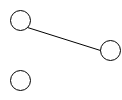
\includegraphics[scale=1]{1}
	\par
\end{center}%
\end{minipage}\hfill{}%
\begin{minipage}[t]{0.5\columnwidth}%
\begin{center}
	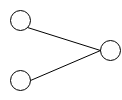
\includegraphics[scale=1]{2}
	\par
\end{center}%
\end{minipage}\linebreak{}
\end{figure}

Ясно, что в таких графах любое наибольшее по включению паросочетание будет максимальным.

\item А вот граф на четырех вершинах существует, он и будет минимальным.

\begin{center}
	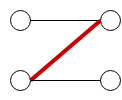
\includegraphics[scale=1]{3}
	\par
\end{center}%

Видно, что выделенное красным паросочетание является наибольшим по включению, но не максимальным: в этом графе существует совершенное паросочетание (черные ребра).

\end{itemize}

\paragraph{7.7} \textit{Имеется колода из $nm$ карт, по одной карте для каждого значения масти из $[m]$ и для каждого значения достоинства из $[n]$. Карты разложены в таблицу с $n$ строками и $m$ столбцами, по одной карте в каждой ячейке. Докажите, что можно найти $m$ карт, которые имеют разные масти и лежат в разных столбцах.}

Построим двудольный граф $K_{x,y}$, где вершины в левой доле ($X$) - будут обозначать номера столбцов, а вершины в правой ($Y$) - масти. Каждую пару вершин $(x, y)$ соеденим $p$ кратными ребрами, где $p$ - число раз, которое показывает сколько раз масть $y$ встретилась в столбце $x$. \textit{Кстати, так как каждая колонка содержит $n$ карт, а каждая масть представлена $n$ достоинствами, то получится $n$-регулярный двудольный граф.}

Формализуем требование задачи: чтобы доказать, что можно найти $m$ карт, которые имеют разные масти и лежат в разных столбцах, достаточно доказать, что в нашем графе существует $X$-насыщенное паросочетание.

Применим теорему Холла: выберем какое-нибудь подможество колонок $U \in X, |U|=k$. В $k$ колонках лежит ровно $nk$ карт. А так как существует $n$ карт каждой масти, то множество $U$ содержит по меньшей мере $k$ различных мастей. Иными словами, $k = |U| \leqslant |N(U)| \leqslant k$.

Условия теоремы Холла выполнены, значит $X$-насыщенное паросочетание найдется, а значит, можно найти $m$ карт, которые имеют разные масти и лежат в разных столбцах.

\end{document}
